\subsection{Apache Flink}
Apache Flink is a large-scale data processing engine optimal to process large amounts of data. It offers APIs for Java, Scala and hadoop MapReduce as well as various APIs to access data. Flink programs can be run locally on a single machine or on a cluster of multiple nodes. When ran on cluster, load distribution and fault tolerance are handled by Apache Flink independently with few configuration effort. Flink enables processing huge amount of data while offering an easy to use API for programmers to implement algorithms.

\subsection{Web Data Commons}
The Web Data Commons is project of the University of Mannheim which is supported by the European Union, Amazon Web Services in Education Grant Award and by the German Research Foundation (DFG). The project offers data sets of the web graph to the public. The data sets were extracted from the Common Crawl Foundation which provides a web corpus to the public.

\subsection{Data sets}
There are multiple data sets offered by the Web Data Commons project differed by year and aggregation level. They offer the Hyperlink Graph 2012 and Hyperlink Graph 2014. Due to different crawling strategies which were used to gather the web corpora, the authors suggest to use the Hyperlink Graph 2012 for comprehensive network analysis of the web graph.

For the Hyperlink Graph 2012 there are the following four different aggregation levels. Page Graph, Subdomain/Host Graph, 1st Subdomain Graph and Pay-Level Domain Graph (PLD).

The Page-Level Graph represents every web page with all details as single node in the graph. An example for a node in this graph would be: dima.tu-berlin.de/menue/database\_ systems\_ and\_ information\_ management\_ group/

The Host Graph aggregates the Page Graph by the subdomains and hosts. Therefore, each subdomain is represented as node within the Host Graph. The two pages tu-berlin.de and dima.tu-berlin.de are two different nodes within this graph.

The PLD reduces the Host Graph by merging the subdomains with their host. The two nodes tu-berlin.de and dima.tu-berlin.de are represented in the PLD as a single node tu-berlin.de.

It is obvious that the size of the graphs decreases with the increase of the granularity level. The graphs are separated into two different files, namely an index file and an arc file. The index file consists of tuples which hold an identifier and the node name. The arc file gives tuples of two identifiers representing a link from one node to another. An overview of the different sizes is given by the following table.

\begin{table}[H]
	\caption{Number of Nodes and Arcs}
	\label{t2}
	\begin{center}
		\begin{tabular}{|l|l|l|}
			\hline
			Data Set	&\#Nodes	&\#Arcs \\ \hline
			Page Graph	&1,727M	&64,422M	\\	\hline
			Subdomain/ Host Graph	&22M	&123M	\\	\hline		
			PLD Graph	&13M	&56M	\\	\hline				
		\end{tabular}
	\end{center}
\end{table}

\subsection{Computation}
We initially planned to run the computations of the algorithms on a ten node cluster. Therefore, we initially intended to use the Host Graph as data set to achieve a comprehensive  analysis of the web graph. Unfortunately, due to organizational problems we were not able to run the computation on the cluster.

As a fallback plan, we decided to run the computation locally on our machines. Very first steps however, revealed that computing these amount of data on a single machine is not feasible, since our machines do not have enough memory. Hence, we reduced the data set to the PLD. This reduction allowed us to compute the indegree distribution and the Top-K outdegree of the PLD. These results were achieved on a machine with 3GB RAM and 2 processors with 2 cores. The computation took around 40 minutes. 

Other implemented algorithms such as the PageRank, closeness and betweenness could not be executed since our machines ran out of memory during the computation.

During the course of the project we were able to run the algorithms on a four node cluster. A detailed view on the configuration of the four node cluster can be seen in Figure \ref{fig6a}. This time we used the Host Graph as well as the PLD Graph as fallback. The computation of the indegree and outdegree was successful on the four node cluster. For both graph levels we were able to retrieve results. Nevertheless, the other algorithms to measure the connectivity, PageRank and closeness of the graph faced memory issues on the four node cluster.

\begin{figure}[H]
	\begin{center}
		\label{fig6a}		
		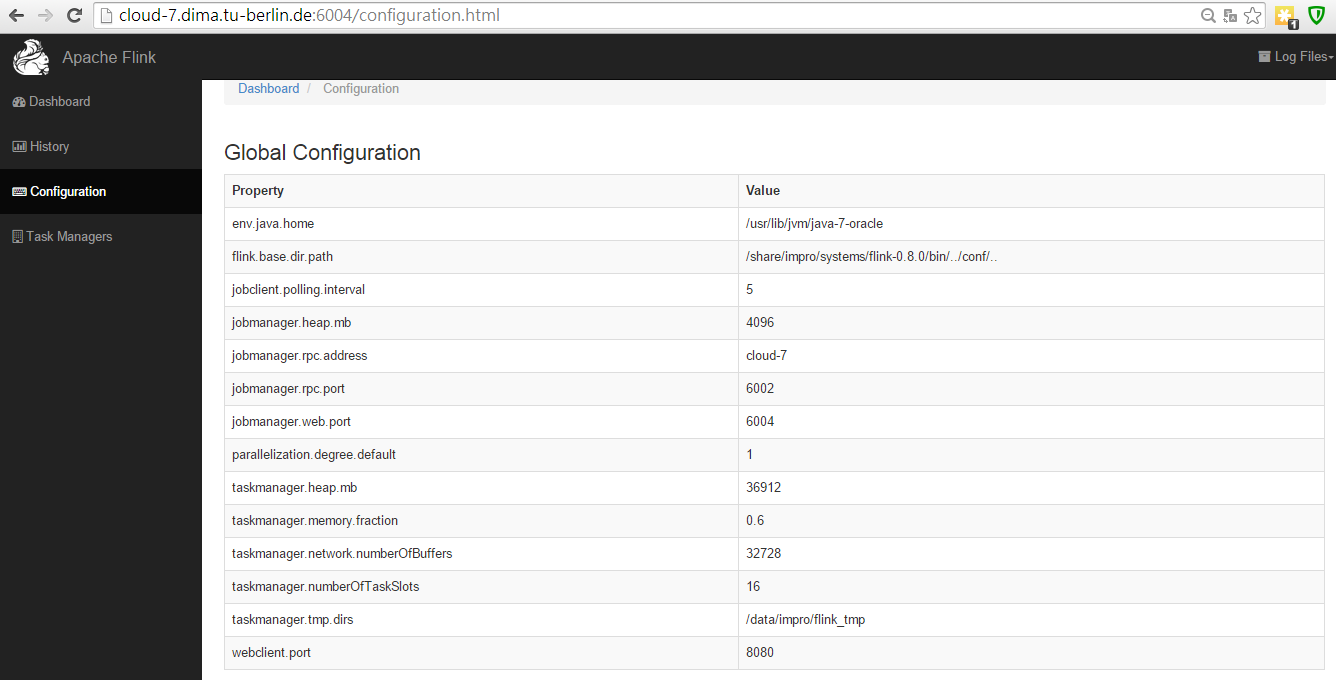
\includegraphics[width=1.0\textwidth]{fig6a}	
		\caption{Configuration of the 4-node cluster}	
	\end{center}
\end{figure}

\begin{table}[H]
	\caption{Computation overviews}
	\label{t3}
	\begin{center}
		\begin{tabular}{|l|l|l|l|}
			\hline		
				&Example graph (locally)	&PLD graph	&Subdomain-Host graph \\ \hline
			Degree	&Correct	&Correct	&Correct \\ \hline
			Connectivity	&Correct	&Memory issue	&Memory issue	\\ \hline
			PageRank	&Correct	&Memory issue	&Memory issue	\\ \hline
			Closeness	&Correct	&Memory issue	&Memory issue	\\ \hline
			Betweenness	&Correlation is 0	&Not run in cluster	&Not run in cluster	\\ \hline
		\end{tabular}
	\end{center}
\end{table}

\subsection{Evaluation}
To rapidly test our implementations of the different algorithms we used an example data set provided by the Web Data Commons project. This data set contains 106 nodes and 141 arcs. The Web Data Commons project provides results for the indegree and outdegree (see Figure 7 and 8). A comparison to these results show that our implementation in respect to the indegree and outdegree is correct and computes the expected results.

\begin{figure}[H]
\begin{minipage}{.5\textwidth}
	\begin{center}
		\label{fig7}		
		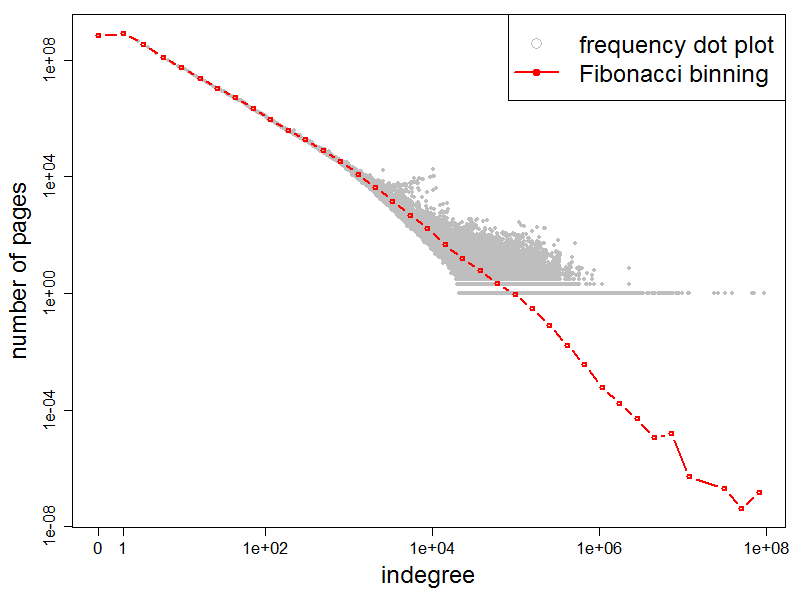
\includegraphics[width=1.0\textwidth]{fig7}	
		\caption{Indegree Distribution}	
	\end{center}
\end{minipage}
\begin{minipage}{.5\textwidth}
	\begin{center}
		\label{fig8}		
		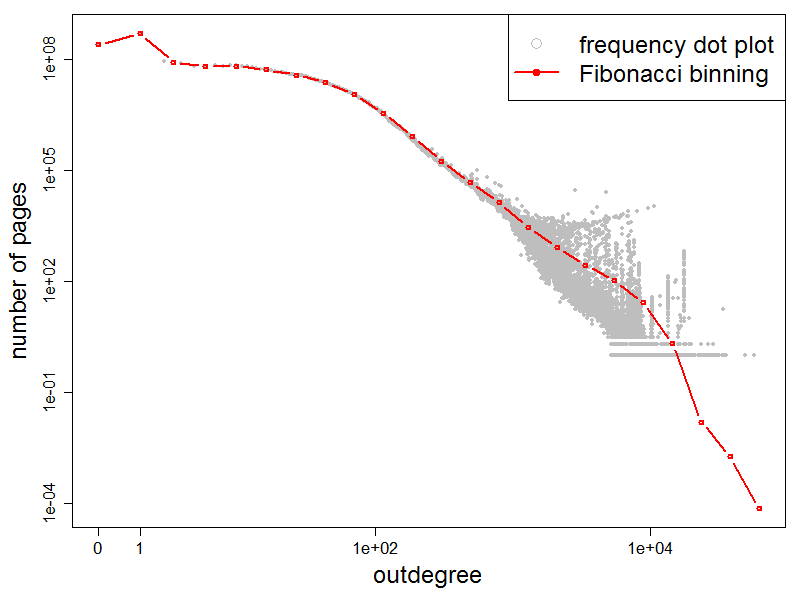
\includegraphics[width=1.0\textwidth]{fig8}	
		\caption{Outdegree Distribution}	
	\end{center}
\end{minipage}
\end{figure}

Further, we used the graph visualization tool Gephi which also provides computation functionalities for the measures degree, PageRank and closeness of graph. We compared our results to the results of Gephi and computed the Pearson correlation between the two result sets.
The correlation coefficient of the two different PageRank results is 1 (see Figure \ref{fig9}). The correlation coefficient for the Closeness results is 0.985 (see Figure \ref{fig10}). This shows that our implementation of the algorithms computes correct results.

\begin{figure}[H]
\begin{minipage}{.5\textwidth}
	\begin{center}
		\label{fig9}		
		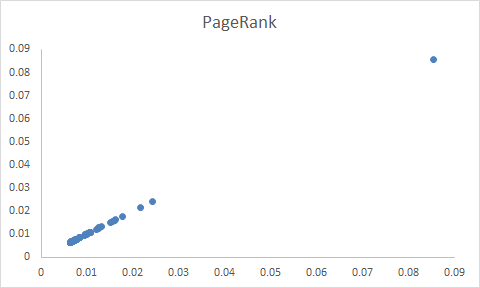
\includegraphics[width=1.0\textwidth]{fig9}	
		\caption{Correlation our results Gephi’s results (PageRank)}	
	\end{center}
\end{minipage} %
\begin{minipage}{.5\textwidth}
	\begin{center}
		\label{fig10}		
		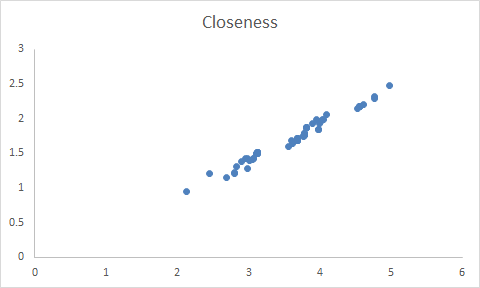
\includegraphics[width=1.0\textwidth]{fig10}	
		\caption{Correlation our results Gephi’s results (Closeness)}	
	\end{center}
\end{minipage}
\end{figure}

\section{Results}
The results of our computation are very limited due to the lack of computation power. We retrieved results from the computation of the indegree and outdegree which can be seen in Figure \ref{fig12} and Figure \ref{fig13}. Since these are our only results, we try to gain as much information from it as we can. Nevertheless, the results of our indegree distribution show the power-law. Yet, tt is observable that the, whether indegree distribution nor the outdegree distribution do not follow a strict linear regression, therefore, we applied  a regression ANOVA to confirm or reject the significance of a power-law.

\begin{figure}[H]
\begin{minipage}{.5\textwidth}
	\begin{center}
		\label{fig12}		
		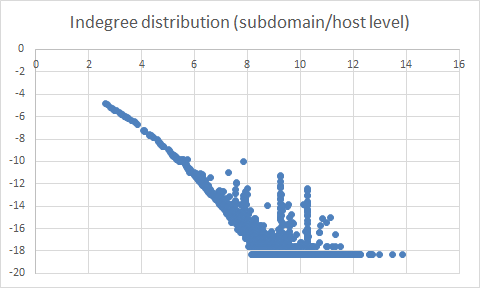
\includegraphics[width=1.0\textwidth]{fig12}	
		\caption{Indegree distribution}	
	\end{center}
\end{minipage} %
\begin{minipage}{.5\textwidth}
	\begin{center}
		\label{fig13}		
		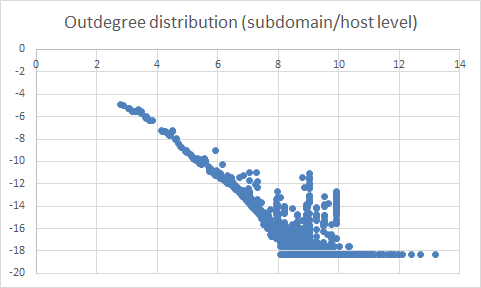
\includegraphics[width=1.0\textwidth]{fig13}	
		\caption{Outdegree distribution}	
	\end{center}
\end{minipage}
\end{figure}

The regression ANOVA (see Figure \ref{fig14}) reveals that the p-value is significant which is 0. However, one of the residual plots, which is the relationship between fitted value (predicted value) and residual, indicates the line is not a regression line (see Figure \ref{fig15}). The reason there is that the residuals have patterns, which violates the assumption of regression that the residuals must have no patterns. Besides, the data also does not follow the assumption that should be normal distribution based on the probability graph. In conclusion, the power-law is not significant. We can therefore confirm the results of other research [4].

\begin{figure}[H]
\begin{minipage}{.5\textwidth}
	\begin{center}
		\label{fig14}		
		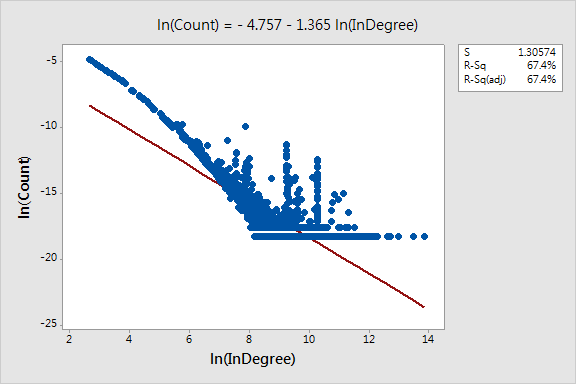
\includegraphics[width=1.0\textwidth]{fig14}	
		\caption{Regression ANOVA}	
	\end{center}
\end{minipage} %
\begin{minipage}{.5\textwidth}
	\begin{center}
		\label{fig15}		
		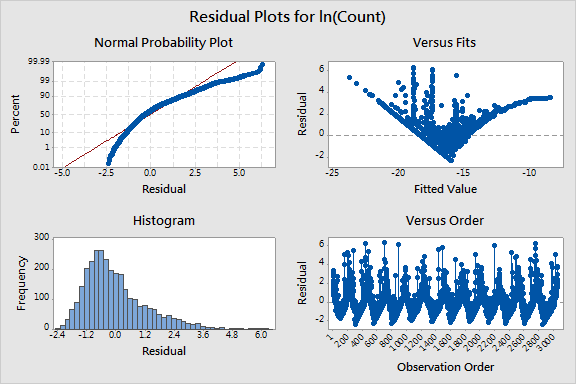
\includegraphics[width=1.0\textwidth]{fig15}	
		\caption{Residual Plots}	
	\end{center}
\end{minipage}
\end{figure}

The results of our Top-10 indegree computation can be seen in Table \ref{t4a}. Further, see Table \ref{t4} for the results of our Top-10 outdegree computation. These results are also confirmed by the Web Data Commons project \footnote{Topology of the 2012 WDC Hyperlink Graph. URL: http://webdatacommons.org/hyperlinkgraph/2012-08/topology.html\#toc9 Last accessed: 10th of February 2015}.

\begin{table}[H]
	\caption{Top-10 Indegree (Host Graph)}
	\label{t4a}
	\begin{center}
		\begin{tabular}{|l|l|}
			\hline
			Website	&Indegree \\ \hline
			wordpress.org	&2,335,856 \\ \hline
			youtube.com	&2,073,535 \\ \hline
			gmpg.org	&1,784,793 \\ \hline
			en.wikipedia.org	&1,545,864 \\ \hline
			twitter.com	&1,036,611 \\ \hline
			google.com	&798,348 \\ \hline
			rtalabel.org	&657,414 \\ \hline
			wordpress.com	&646,766 \\ \hline
			mp3shake.com	&549,122 \\ \hline
			w3schools.com	&507,184 \\ \hline
		\end{tabular}
	\end{center}
\end{table}

\begin{table}[H]
	\caption{Outdegree and Page views}
	\label{t4}
	\begin{center}
		\begin{tabular}{|l|l|l|}
			\hline
			Website	&Outdegree	&Page views \\ \hline
			serebella.com	&699609	&3 \\ \hline
			tumblr.com	&496045	&7.18 \\ \hline
			blogspot.com	&3898561	&3.21 \\ \hline
			wordpress.com	&2249553	&4.71 \\ \hline
			refertus.info	&668271	&1 \\ \hline
			typepad.com	&551360	&1.89 \\ \hline
			botw.org	&496645	&2.82 \\ \hline
			top20directory.com	&650884	&1.3 \\ \hline
			wikipedia.org	&862705	&3.53 \\ \hline	
			youtube.com	&1078938	&6.08 \\ \hline			
		\end{tabular}
	\end{center}
\end{table}